\chapter{Machine Learning Models}

\section{Introduction}
As explained in dept in the methodology chapter, the biometric data collected through the watches generated a total of 6 independent variables:

\begin{itemize}
    \item Heart Rate Maximum \textit{bm\_HR\_max}
    \item Heart Rate Average \textit{bm\_HR\_avg}
    \item Heart Rate Variability \textit{bm\_HR\_var}
    \item Activity Steps \textit{bm\_act\_steps}
    \item Sleep \textit{bm\_sleep}
\end{itemize}

The dependent variables that were collected through the gaming tests are:

\begin{itemize}
    \item Fine Motor Tracking Time \textit{fm\_avg\_trk\_time}
    \item Fine Motor Accuracy \textit{fm\_accuracy}
    \item Visual Average Response Time \textit{vx\_avg\_res\_time}
    \item Visual Shot Accuracy \textit{vx\_shot\_accuracy}
    \item Visual Target Accuracy \textit{vx\_trg\_accuracy}
    \item Audio Average Response Time \textit{au\_avg\_res\_time}
\end{itemize}

The goal based on the research question was to find the correlation between the independent and dependent variables. When approaching a machine learning problem, one of the fundamental
considerations is wheter the problem is a regression or classification problem. 

\subsection*{Classification Problem}
Classification is used when the dependent variable is categorical, meaning it can take one of a limited number of values. Examples includes predicting whether an email is spam or not,
whether a patient has a disease or not, whether a customer will buy a product or not. 

\subsection*{Regression Problem}
Regression is used when the dependent variable is continuous and numerical, meaning it can take any value within a range. Examples includes predicting house prices, stock prices, 
temperature. In this project, the dependent variables are continuous and numerical, making it a regression problem. The goal was to predict the dependent variables based on the biometric
data collected from the watches. 

\section{Data Exploration}
The first step in the machine learning process was to explore the dataset. The dataset was loaded into a pandas dataframe and the first 5 rows were displayed to get an overview of the
data. The shape of the dataset was checked to see the number of rows and columns. The data types of the columns were checked to ensure that the data types were correct. The summary
statistics of the dataset were checked to see the mean, median, standard deviation, minimum and maximum values of the dataset. The correlation between the independent and dependent
variables were checked to see if there was any correlation between the variables. The correlation was visualized using a heatmap \ref{fig:correlation_heatmap} to see the correlation 
between the variables.

\begin{figure}[H]
    \centering
    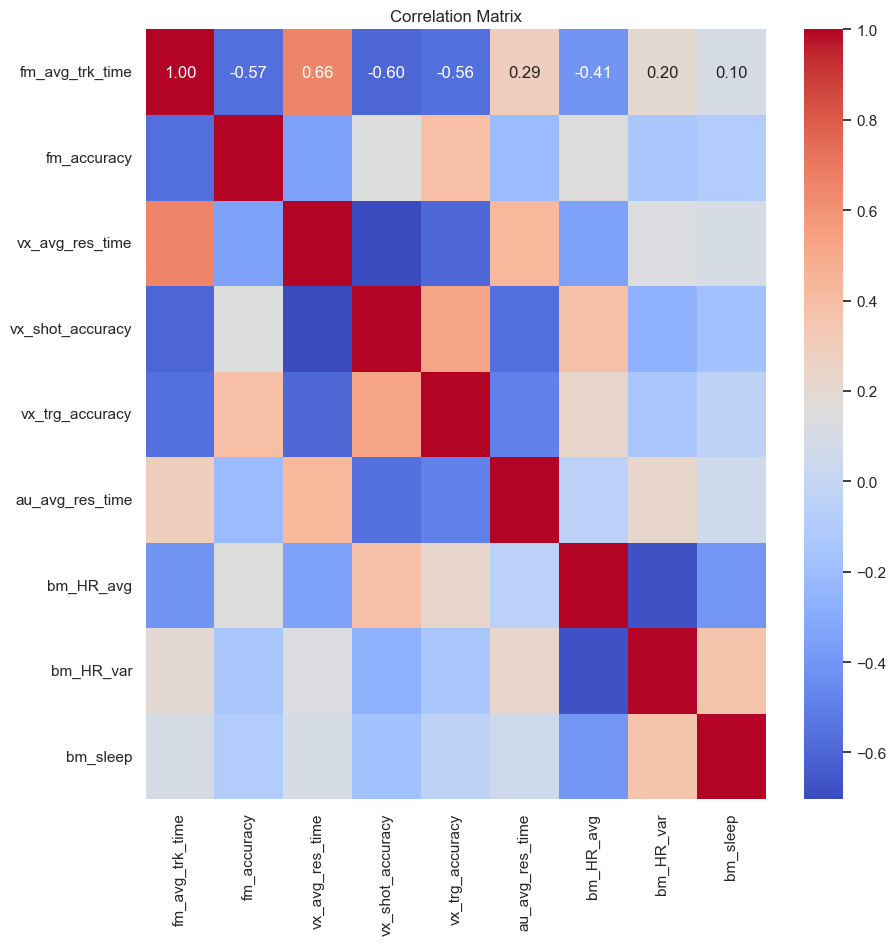
\includegraphics[width=1\textwidth]{images/correlation.png}
    \caption{Correlation Heatmap}
    \label{fig:correlation_heatmap}
\end{figure}

From the correlation heatmap, it can be seen that there is are some variables that are highly correlated with each other. Below are the variables that are highly correlated with each other:

\begin{itemize}
    \item Fine Average Tracking Time and Visual Average Response Time: Strong positive correlation (0.66), suggesting that as the Fine motor average tracking time increases, 
    the Audio average response tends to increases.
    \item Fine Motor Average Tracking Time and Sleep: Not a strong correlation (0.10), which could imply that higher the sleep time, the higher the fine motor average tracking time.
    \item Visual Average Response Time and Sleep: A correlation of (0.20), indicates a slight tendency for a higher visual response time to be associated with higher sleep time.
    \item Visual Shot Accuracy and Audio Average Response Time: A correlation of (0.29), suggests a slight tendency that higher Visual shot accuracy is associated with faster 
    \item Heart Rate Average and Sleep
\end{itemize}



\section{Data Pre-processing}
To have the dataset suitable for the machine learning models, the data was pre-processed. It was found that were many null values that needed to be handled, 
it was removed from the dataset as it was not possible to impute the values. The \section{Activity Steps} and \section{Heart Rate Maximum} were found to have
outliers that were removed from the dataset. The data was then scaled using StandardScaler from the sklearn library. This was done to ensure that all the features
contribute equally to the result.
The columns \textit{\_id}, \textit{\_date} and \textit{\_user} were removed from the dataset as they were not needed for the machine learning models.


\section{Model Selection and Evaluation}
Various machine learning models were explored to address the research question and predict the dependent variables based on the collected biometric and gaming test. Each team member
focused on developing and evaluating a model to achieve the best predictive performance. 


\section{Classical ML Regression Model}
The first model that was explored was the classical machine learning regression model. The model was trained using the training dataset and evaluated using the testing dataset. 
The model was evaluated using the mean squared error. The model was trained using the following algorithms:

\begin{itemize}
    \item Linear Regression: Chose as a baseline for its simplicity and interpretability, assuming a linear relationship between the dependent and independent variables.
    \item Random Forest Regressor: Chose for its ability to handle non-linear relationships and its robustness to overfitting. 
    \item Support Vector Regressor: Selected for its ability to handle high-dimensional data and capability to find complex patterns by mapping input data into a higher-dimensional feature space.
    \item K-Nearest Neighbours Regressor: Chose for its simplicity and effectiveness in regression tasks, making predictions based on the average of the k-nearest neighbours in the feature space.
\end{itemize}

Each model was trained on pre-processed data and evaluated using the standard regression performance metric mean squared error (MSE). The best performing model for each variable was 
identified utilized for further analysis.




\section{Neural Network Regression Model}



